% This is samplepaper.tex, a sample chapter demonstrating the
% LLNCS macro package for Springer Computer Science proceedings;
% Version 2.20 of 2017/10/04
%
\documentclass[runningheads]{llncs}
%
\usepackage{lipsum}
\usepackage{pgfplots}
\usepackage{subcaption}
\usepackage{caption}

\usepackage{cmap}
\usepackage[utf8]{inputenc}
\usepackage[T2A]{fontenc}
\usepackage[russian]{babel}

\usepackage{graphicx}
% Used for displaying a sample figure. If possible, figure files should
% be included in EPS format.
%
% If you use the hyperref package, please uncomment the following line
% to display URLs in blue roman font according to Springer's eBook style:
% \renewcommand\UrlFont{\color{blue}\rmfamily}

\begin{document}
%
\title{Разработка библиотеки для хранения временных рядов с помощью LSM дерева на языке
	программирования Go}
%
%\titlerunning{Abbreviated paper title}
% If the paper title is too long for the running head, you can set
% an abbreviated paper title here
%
\author{Никита Томилов\orcidID{0000-0001-9325-0356}}
%
\authorrunning{Никита Томилов}
% First names are abbreviated in the running head.
% If there are more than two authors, 'et al.' is used.
%
\institute{Университет ИТМО, Санкт-Петербург, Россия \\
\email{mr@itmo.ru}\\
\url{http://micsecs.org/}}
%
\maketitle              % typeset the header of the contribution
%
\begin{abstract}
Due to the recent growth in popularity of the Internet of Things solutions, the amount of data being captured, stored, and transferred is also significantly increasing. The concept of edge devices allows buffering of the time-series measurement data to help mitigating the network issues. 
One of the options to safely buffer the data on such a device within the currently running application is to use some kind of embedded database. However, those can have poor performance, especially on embedded computers. It may lead to bigger response times, which can be harmful for mission-critical applications. That is why in this paper an alternative solution, which involves the LSM tree data structure, was advised.
The article describes the concept of an LSM tree-based storage for buffering time series data on an edge device within the Golang application. To demonstrate this concept, a GoLSM library was developed. Then, a comparative analysis to a traditional in-application data storage engine SQLite was performed. This research shows that the developed library provides faster data reads and data writes than SQLite as long as the timestamps in the time series data are linearly increasing, which is common for any data logging application.

\keywords{Временные ряды \and LSM дерево \and SST \and Golang.}
\\
Перевод с английского языка.
\end{abstract}
%
%
%
\section{Theoretical background}
\subsection{Time Series data}
Typically, a time series data is the repeated measurement of parameters over time together with the times at which the measurements were made~\cite{time_series_databases}. Time series often consist of measurements made at regular intervals, but the regularity of time intervals between measurements is not a requirement. As an example, the temperature measurements for the last week with the timestamp for each measurement is a time series temperature data. The time series data is most commonly used for analytical purposes, including machine learning for predictive analysis. A single value of such data could be both a direct measurement from a device or some calculated value, and as long as it has some sort of timestamp to it, the series of such values could be considered a time series.

\subsection{IoT data and Edge computing}
Nowadays the term "time-series data" is well-known due to the recent growth in popularity of the Internet of Things, or IoT, devices, and solutions, since an IoT device is often used to collect some measure in a form of time-series data. Often this data is transferred to a server for analytical and statistical purposes. However, in a large and complex monitoring system, such as an industrial IoT, the amount of data being generated causes various problems for transferring and analyzing this data. A popular way of extending the capabilities of IoT system is to introduce some form of intermediate devices called "edge" devices~\cite{ind_iot_edge}. The traditional architecture of organizing a complicated IoT system is shown in Figure~\ref{fig1}.

\begin{figure}[htb]
\centering
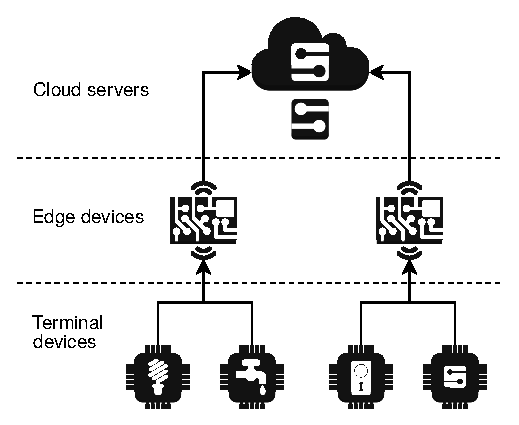
\includegraphics{figures/iot-hierarchy.drawio.eps}
\caption{An architecture of a complicated IoT system.} \label{fig1}
\end{figure}

This architecture provides flexibility in terms of data collection.
In case of problems with the network connection between the endpoint device and the cloud, data can be buffered in the edge device and then re-sent to the server when the connection is established. Therefore, an edge device should have the possibility to accumulate the data from the IoT devices for those periods of the network outage. However, often an edge device is not capable to run a proper database management system apart from other applications. So there has to be a way to embed the storing of time-series data to an existing application. From this point we will assume the application is written in a Go programming language because this language maintains the balance between complexity, being easier to use than C/C++, and resource inefficiency, being less demanding than Python.

\subsection{In-app data storage}
Traditionally, either some form of in-memory data structures or embedded databases are used to store data within the application. However, if data is critical and it is important not to lose it in case of a power outage, in-memory storage doesn't fit. An embedded database or other forms of persistent data storage that is used within the application, reduce the access speed compared to any in-memory storage system. This article describes an LSM-based storage system. This type of system is providing the best of both worlds - persistent data storage with fast data access.
\section{Implementation}
\subsection{LSM tree}
An LSM tree, or log-structured merge-tree, is a key-value data structure with high-performance characteristics. It is a good choice for providing indexed access to the data files, such as transaction log data or time series data. LSM tree maintains the data in two or more structures. Each of them is optimized for the media it is stored on, and the synchronization between the layers is done in batches~\cite{lsm_tree_orig}.

A simple LSM tree consists of two layers, named $C_0$ and $C_1$. The main difference between these layers is that typically $C_0$ is an in-memory data structure, while $C_1$ should be stored on a disk. Therefore, $C_1$ usually is bigger than $C_0$, and when the amount of data in $C_0$ reaches a certain threshold, the data is merged to $C_1$. To maintain a suitable performance it is suggested both $C_0$ and $C_1$ have to be optimized for their application. The data has to be migrated efficiently, probably using algorithms that may be similar to merge sort.

To maintain this merging efficiency, it was decided to use SSTable as the $C_1$ level, and B-tree for the $C_0$. SSTable, or Sorted String Table, is a file that contains key-value pairs, sorted by key~\cite{sstable}. Using SSTable for storing time series data is a good solution if the data is being streamed from a monitoring system. Because of this, they are sorted by the timestamp, which is a good candidate for the key. The value for the SSTable could be the measurement itself. SSTable is always an immutable data structure, meaning that the data cannot be directly deleted from the file; it has to be marked as "deleted" and then removed during the compaction process. The compaction process is also used to remove the obsolete data if it has a specific time-to-live period.

\subsection{Commitlog}
Any application that is used to work with mission-critical data has to have the ability to consistently save the data in case of a power outage or any other unexpected termination of the application. To maintain this ability, a commit log mechanism is used. It is a write-only log of any inserts to the database. It is written before the data is appended to the data files of the database. This mechanism is commonly used in any relational or non-relation DBMS.

Since the in-app storage system has to maintain this ability as well, it was necessary to implement the commit log alongside the LSM tree. In order to ensure the entries in this commit log are persisted on the disk storage, the fsync syscall was used, which negatively affected the performance of the resulted storage system.

\subsection{Implemented library}
In order to implement the feature of storing time-series data within the Go application, it was developed the GoLSM library. It provides mechanisms to persist and retrieve time-series data, and it uses a two-layer LSM tree as well as a commit log mechanism to store the data on disk. The architecture of this library is represented in Figure~\ref{fig2}.
\begin{figure}[h!]
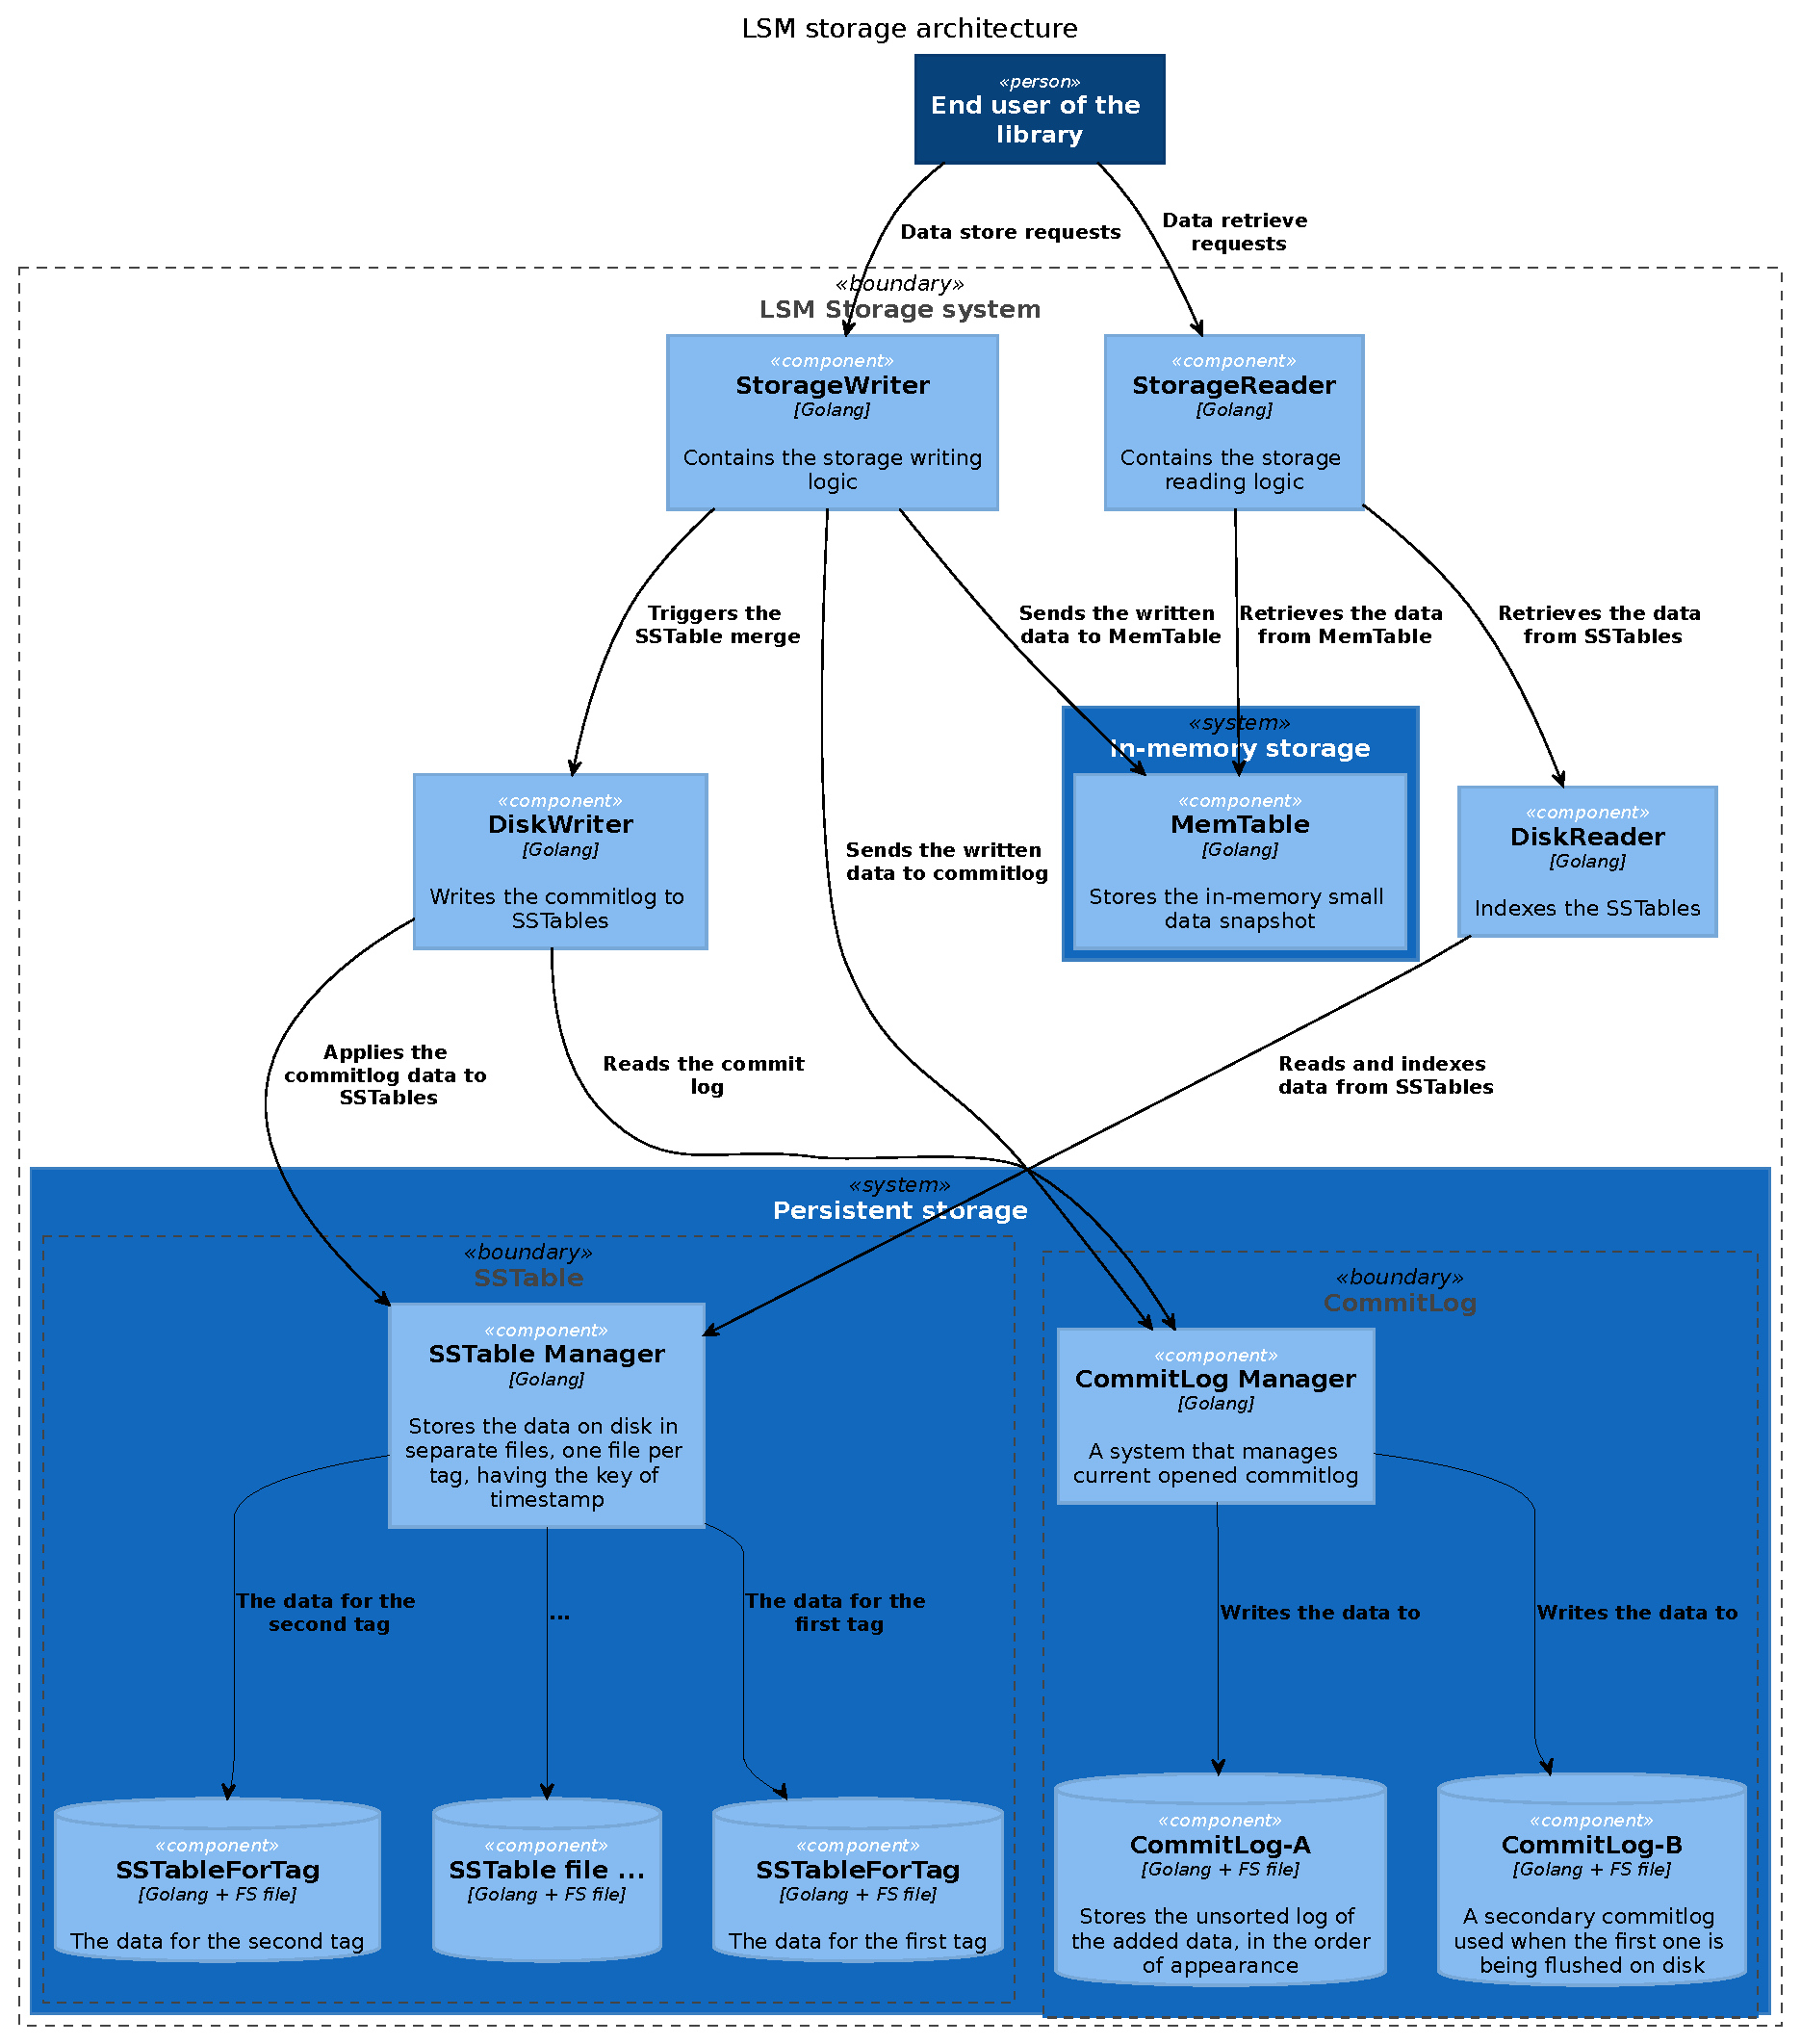
\includegraphics[width=\textwidth,keepaspectratio]{figures/golsm-arch.eps}
\caption{An architecture of a GoLSM library.} \label{fig2}
\end{figure}

 Since this library was initially developed for a particular subject area and particular usage, it has a number of limitations. For example, it has no functions to delete the data; instead, it is supposed to save the measurement with a particular expiration point, after which the data will be automatically removed during the compaction process. The data are storing with GoLSM should consist of one or multiple measurements; each measurement is represented by a tag name, which could be an identifier of a sensor or the measurement device, origin, which is the timestamp when the measurement was captured, and the measurement value, which is stored as a byte array. This byte array can vary in size. It makes the storage of each measurement a more complicated procedure.

As seen, the storage system consists of two layers, in-memory layer and persistent storage layer. The in-memory layer is based on a B-tree implementation by Google~\cite{btree_google} . It stores a small portion of the data of a configurable size. The storage layer consists of a commit log manager and an SSTable manager. The commit log manager maintains the two commit log files; while one is used to write the current data, another one is used to append the previously written data to the SSTables, which are managed by SSTable Manager. Each SSTable file contains its own tag, and it also has a dedicated in-memory index, which is also based on a B-tree. This index is used to speed up the retrieval of the data from the SSTable when the requested time range is bigger than what is stored on an in-memory layer.
\section{Сравнение с SQLite}

\subsection{Методология сравнения}

Для сравнения LSM-решения с SQLite была разработана простая система хранения на основе SQLite. Она использует базу данных, состоящую из двух таблиц. Первая таблица называется Measurement и используется для хранения измерений. Каждое измерение представлено своим ключом, временной меткой и значением, а ключ - это первичный идентификатор объекта MeasurementMeta, который хранится во второй таблице. Этот объект хранит имя тега измерения; поэтому можно выполнять поисковые операции с фильтрацией по числовому столбцу вместо текстового столбца. В таблице измерений есть индексы как для ключевого столбца, так и для столбца временной метки.

Для следующих тестов использовалась придуманная синтетическая система. Эта система имеет 10 датчиков, которые производят данные с частотой дискретизации 1 Гц. Для тестов чтения данные для этих 10 тегов были сгенерированы для трех часов измерений. Следовательно, в базе данных SQLite содержатся 108000 записей или точек, или 10800 точек на каждый тег. Библиотека LSM также содержит 108000 записей, разделенных на 10 файлов для каждого тега, по 10800 точек в каждом. Для тестов записи данные для этих 10 тегов генерируются для различных временных диапазонов и затем сохраняются в обоих механизмах хранения.

Для тестирования обоих механизмов хранения использовался стандартный механизм тестирования Go. Он запускает целевой код несколько раз, пока тестовая функция не проработает достаточно долго, чтобы время ее выполнения можно было надежно измерить ~\cite {go_benchmark}. Этот механизм дает результат, который измеряется в ns/op, наносекундах на итерацию; для данных тестов итерация - это один вызов чтения или записи в хранилище.

Все тесты выполнялись на ПК с Intel Core i5-8400 под управлением Ubuntu 18.04, файлы данных для обоих хранилищ хранились на твердотельном накопителе NVMe.

\subsection{Чтение всего диапазона данных}

Этот тест измеряет время считывания для различных временных диапазонов, в то время как операция выполняется для полных трех часов измерений. Результаты этого теста представлены на рисунке ~\ref{fig3}. Как видно, GoLSM примерно в два раза быстрее SQLite по запросам на чтение. Стоит отметить, что уровень $C_0$ LSM-дерева не играет существенной роли в ускорении извлечения данных, поскольку временной диапазон выбирается случайным образом из всех трех часов измерений, в то время как уровень $C_0$ содержит только последние две минуты измерений.

\begin{figure}[h!]
	\centering
	\begin{tikzpicture}
        % first provide your data as table, so later the data can
        % easily be accessed for various stuff
        \pgfplotstableread{
            x    y  z
5 29245				    2468624
10 34331			    2488443
15 41885			    2487442
20 47359			    2533488
25 51261			    2517353
30 62037			    2529031
45 76538			    2571565
60 101490			    2611909
120 185574			    2787438
180 241142			    2986666
240 341329			    3155070
300 412849			    3327132
600 801901			    4190652
900 1264738			    5008636
1200 1549898			    5966411
1500 1895210			    6753930
1800 2550300			    7420697
2700 3659991			    10027510
3600 5442224			    12570023
4500 6261830			    15128483
5400 7410561			    16932040
6300 8529041			    19965360
7200 10960360			    22752193
8100 12106688			    24262132
        }{\data}
    \begin{axis}[
        x tick style={/pgf/number format/1000 sep=},
	    ylabel style={align=center},	
	    ylabel = \textbf{Ns/op}\\lower is better,
	    xlabel style={align=center},	
	    xlabel = \textbf{Requested time range, seconds},
	    enlargelimits=0.05,
	    legend style={
	        at={(0.5,1.1)}, anchor=north,legend columns=-1
	    },
    ]
        % then your `\addplot commands change to
        \addplot table [x=x,y=y] {\data};
        \addlegendentry{GoLSM}
        \addplot table [x=x,y=z] {\data};
        \addlegendentry{SQLite}
    \end{axis}
\end{tikzpicture}
	\caption{Чтение всего диапазона данных.} \label{fig3}
\end{figure}

Как видно, хранилище LSM до 50 раз быстрее, чем SQLite в небольшом диапазоне запросов (51251 нс/операцию для GoLSM и 2517353 нс/операцию для SQLite в диапазоне 25 секунд) и до двух раз быстрее в большом диапазоне запросов (12106688 нс/оп и 24262132 нс/оп в диапазоне 2 ч 15 мин). Эта большая разница может быть вызвана использованием индекса в памяти для каждого файла SST, который работает лучше, чем индексация в SQLite. Повышение эффективности для малого диапазона запросов может быть вызвано тем фактом, что малый запрошенный диапазон с большей вероятностью умещается в пределах уровня $C_0$ дерева LSM, поэтому медленное извлечение из SST не вызывается.

\subsection{Чтение за последние три минуты}

Этот тест измеряет время считывания для различных временных диапазонов, в то время как операция выполняется для последних трех минут измерений. Результаты этого теста показаны на рисунке ~\ref{fig4}. Поскольку уровень $C_0$ LSM-дерева содержит последние две минуты измерений, более вероятно, что запрос будет соответствовать уровню $C_0$ без необходимости запрашивать данные с уровня $C_1$. Таким образом, извлечение данных в два раза быстрее, чем извлечение данных за все три часа измерений, как показано на рисунке ~\ref{fig5}. 

\begin{figure}[!htb]
	\begin{minipage}{0.48\textwidth}
		\centering
		\resizebox{\textwidth}{!}{%
			\begin{tikzpicture}
        % first provide your data as table, so later the data can
        % easily be accessed for various stuff
        \pgfplotstableread{
            x    y  z
5 14164				    2179781
10 18772			    2190392
15 24835			    2222522
20 30221			    2216021
25 33592			    2268216
30 43931			    2253056
45 58727			    2337832
60 84315			    2380516
75 102221			    2393851
90 121761			    2470748
        }{\data}
    \begin{axis}[
        x tick style={/pgf/number format/1000 sep=},
	    ylabel style={align=center},	
	    ylabel = \textbf{Ns/op}\\lower is better,
	    xlabel style={align=center},	
	    xlabel = \textbf{Requested time range, seconds},
	    enlargelimits=0.05,
	    legend style={
	        at={(0.5,1.1)}, anchor=north,legend columns=-1
	    },
    ]
        % then your `\addplot commands change to
        \addplot table [x=x,y=y] {\data};
        \addlegendentry{GoLSM}
        \addplot table [x=x,y=z] {\data};
        \addlegendentry{SQLite}
    \end{axis}
\end{tikzpicture}
		}
		\caption{Чтение всего диапазона данных}\label{fig4}
	\end{minipage}\hfill
	\begin{minipage}{0.48\textwidth}
		\centering
		\resizebox{\textwidth}{!}{%
			\begin{tikzpicture}
        % first provide your data as table, so later the data can
        % easily be accessed for various stuff
        \pgfplotstableread{
            x    y  z
5	29245	14164
10	34331	18772
15	41885	24835
20	47359	30221
25	51261	33592
30	62037	43931
45	76538	58727
60	101490	84315
        }{\data}
    \begin{axis}[
        x tick style={/pgf/number format/1000 sep=},
	    ylabel style={align=center},	
	    ylabel = \textbf{Ns/op}\\lower is better,
	    xlabel style={align=center},	
	    xlabel = \textbf{Requested time range, seconds},
	    enlargelimits=0.05,
	    legend style={
	        at={(0.5,1.1)}, anchor=north,legend columns=-1
	    },
    ]
        % then your `\addplot commands change to
        \addplot table [x=x,y=y] {\data};
        \addlegendentry{GoLSM, full range}
        \addplot table [x=x,y=z] {\data};
        \addlegendentry{GoLSM, last three minutes}
    \end{axis}
\end{tikzpicture}
		}
		\caption{Разница в скорости для разных интервалов.}\label{fig5}
	\end{minipage}
\end{figure}

Если в системе предполагается чтение только самых последних данных, увеличение емкости $C_0$ может значительно улучшить производительность чтения и снизить нагрузку чтения на постоянное хранилище диска.

\subsection{Запись упорядоченных данных}

Этот тест измеряет время записи для различных временных диапазонов. В то время как данные являются упорядоченными, минимальная временная метка следующего записываемого пакета данных всегда больше, чем максимальная временная метка ранее записанного пакета. Это означает, что для каждого SST-файла в GoLSM данные добавляются только в конец SST-файла без необходимости повторять сортировку SST-файла. Результаты этого теста представлены на рисунке ~\ref{fig6}.

\begin{figure}[!htb]
	\begin{minipage}{0.48\textwidth}
		\centering
		\resizebox{\textwidth}{!}{%
			\begin{tikzpicture}
        % first provide your data as table, so later the data can
        % easily be accessed for various stuff
        \pgfplotstableread{
            x    y  z
5 15645901			    9353729
10 22956983			    11181460
15 32283634			    19307910
20 34011973			    21123025
25 33267746			    28927692
30 39930080			    30805858
45 49632256			    47978279
60 54524124			    59648520
120 84668307			    116531430
180 115137807			    173160076
240 146032654			    228964797
300 151417281			    293465746
600 298689957			    592581370
900 452684093			    923305824
1200 587385346			    1249406072
1500 747870163			    1582051745
1800 899311404			    1974174575

        }{\data}
    \begin{axis}[
        x tick style={/pgf/number format/1000 sep=},
	    ylabel style={align=center},	
	    ylabel = \textbf{Ns/op}\\lower is better,
	    xlabel style={align=center},	
	    xlabel = \textbf{Written time range, seconds},
	    enlargelimits=0.05,
	    legend style={
	        at={(0.5,1.1)}, anchor=north,legend columns=-1
	    },
    ]
        % then your `\addplot commands change to
        \addplot table [x=x,y=y] {\data};
        \addlegendentry{GoLSM}
        \addplot table [x=x,y=z] {\data};
        \addlegendentry{SQLite}
    \end{axis}
\end{tikzpicture}
		}
		\label{figure}{(а) Для большого диапазона}
	\end{minipage}\hfill
	\begin{minipage}{0.48\textwidth}
		\centering
		\resizebox{\textwidth}{!}{%
			\begin{tikzpicture}
        % first provide your data as table, so later the data can
        % easily be accessed for various stuff
        \pgfplotstableread{
            x    y  z
5 15645901			    9353729
10 22956983			    11181460
15 32283634			    19307910
20 34011973			    21123025
25 33267746			    28927692
30 39930080			    30805858
45 49632256			    47978279
60 54524124			    59648520
120 84668307			    116531430

        }{\data}
    \begin{axis}[
        x tick style={/pgf/number format/1000 sep=},
	    ylabel style={align=center},	
	    ylabel = \textbf{Ns/op}\\lower is better,
	    xlabel style={align=center},	
	    xlabel = \textbf{Written time range, seconds},
	    enlargelimits=0.05,
	    legend style={
	        at={(0.5,1.1)}, anchor=north,legend columns=-1
	    },
    ]
        % then your `\addplot commands change to
        \addplot table [x=x,y=y] {\data};
        \addlegendentry{GoLSM}
        \addplot table [x=x,y=z] {\data};
        \addlegendentry{SQLite}
    \end{axis}
\end{tikzpicture}
		}
		\label{figure}{(б) Для маленького диапазона}
	\end{minipage}
	
	\caption{Запись упорядоченных данных.}\label{fig6}
\end{figure}

На рисунке ~\ref{fig6}, (а) видно, что GoLSM записывает данные в два раза быстрее, чем SQLite, в течение большого записываемого диапазона времени. Однако на рисунке ~\ref{fig6}, (б) для небольшого временного диапазона GoLSM на самом деле медленнее. Причина этого в том, что для LSM измерялось время до момента фактической записи данных в журнал фиксации, а не непосредственно в файлы SST; и когда количество записей в журнале фиксации достигает определенного порога, оно должно быть передано в SST, что вызывает скачки времени записи. Однако для записываемых больших временных диапазонов эти накладные расходы не важны по сравнению с обычно медленными пакетными вставками в SQLite.

Стоит отметить, что для вставки в SQLite необходимо составить оператор SQL Insert, который включает преобразование значения типа double в строку. Эта операция выполняется очень медленно для больших пакетов вставок (пакет из 10 тегов за 30 минут составляет 18000 точек), и использование ORM, такого как GORM, не улучшает ситуацию.

\subsection{Запись неупорядоченных данных}

Этот тест измеряет время записи для различных временных диапазонов, но, поскольку данные являются неупорядоченными, нет никаких гарантий, что все временные метки следующего пакета больше, чем временные метки ранее записанного пакета. Таким образом, пакеты могут быть получены до или после друг друга с точки зрения их временных меток. Это означает, что каждый раз, когда данные передаются из файла журнала фиксации в файлы SST, библиотека должен пересортировать весь файл SST, замедляя процесс записи. Результаты этого теста представлены на рисунке ~\ref{fig7}. Сравнение записи данных в LSM, когда данные являются упорядоченными или неупорядоченными, доступно на рисунке ~\ref {fig8}.

\begin{figure}[!htb]
	\begin{minipage}{0.48\textwidth}
		\centering
		\resizebox{\textwidth}{!}{%
			\begin{tikzpicture}
        % first provide your data as table, so later the data can
        % easily be accessed for various stuff
        \pgfplotstableread{
            x    y  z
5 20066750			    9514015
10 34790230			    10956443
15 61277403			    19290607
20 66074549			    20865090
25 63925416			    28999975
30 83572878			    30478476
45 94080339			    48656675
60 100926498			    59882936
120 154617448			    117794298
180 218391345			    178663220
240 277609792			    238031796
300 291599762			    299054072
600 633156270			    616109936
900 977887157			    948873690
1200 1364639379			    1293479495
1500 1942545058			    1592474416
1800 2362087783			    2026594877


        }{\data}
    \begin{axis}[
        x tick style={/pgf/number format/1000 sep=},
	    ylabel style={align=center},	
	    ylabel = \textbf{Ns/op}\\lower is better,
	    xlabel style={align=center},	
	    xlabel = \textbf{Written time range, seconds},
	    enlargelimits=0.05,
	    legend style={
	        at={(0.5,1.1)}, anchor=north,legend columns=-1
	    },
    ]
        % then your `\addplot commands change to
        \addplot table [x=x,y=y] {\data};
        \addlegendentry{GoLSM}
        \addplot table [x=x,y=z] {\data};
        \addlegendentry{SQLite}
    \end{axis}
\end{tikzpicture}
		}
		\caption{Запись неупорядоченных данных.}\label{fig7}
	\end{minipage}\hfill
	\begin{minipage}{0.48\textwidth}
		\centering
		\resizebox{\textwidth}{!}{%
			\begin{tikzpicture}
        % first provide your data as table, so later the data can
        % easily be accessed for various stuff
        \pgfplotstableread{
            x    y  z
5	15645901	20066750
10	22956983	34790230
15	32283634	61277403
20	34011973	66074549
25	33267746	63925416
30	39930080	83572878
45	49632256	94080339
60	54524124	100926498
120	84668307	154617448
180	115137807	218391345
240	146032654	277609792
300	151417281	291599762
600	298689957	633156270
900	452684093	977887157
1200	587385346	1364639379
1500	747870163	1942545058
1800	899311404	2362087783

        }{\data}
    \begin{axis}[
        x tick style={/pgf/number format/1000 sep=},
	    ylabel style={align=center},	
	    ylabel = \textbf{Ns/op}\\lower is better,
	    xlabel style={align=center},	
	    xlabel = \textbf{Requested time range, seconds},
	    enlargelimits=0.05,
	    legend style={
	        at={(0.5,1.1)}, anchor=north,legend columns=-1
	    },
    ]
        % then your `\addplot commands change to
        \addplot table [x=x,y=y] {\data};
        \addlegendentry{GoLSM, linear data}
        \addplot table [x=x,y=z] {\data};
        \addlegendentry{GoLSM, random data}
    \end{axis}
\end{tikzpicture}
		}
		\caption{Разница во времени при записи упорядоченных и неупорядоченных данных.}\label{fig8}
	\end{minipage}
\end{figure}

Как видно на рисунке ~\ref {fig7}, накладные расходы на пересортирование файлов SST при каждой записи данных настолько велики, что они занимают больше времени, чем медленные пакетные вставки в SQLite. Сравнение записи данных с этими накладными расходами с записью данных без накладных расходов показано на рисунке ~\ref{fig8}. Когда временные метки данных всегда линейно увеличиваются, это показывает, что вставки почти в три раза медленнее при записи в большом временном диапазоне (747870163 нс/операцию, или 747 мс, для записи 25 минут линейных данных и 1942545058 нс/операцию, или 1942 мс, для записи 25 минут случайных данных).
\section{Conclusion}

As shown in the article, the developed LSM storage library provides faster write and read operations for the time series data than SQLite. Also, it allows keeping data in case of unexpected application crashes due to commit log mechanism. In the best cases, this library is up to 50 times faster than SQLite for read operations, thanks to its $C_0$ level. It effectively serves as an in-memory cache, and up to 2 times faster than SQLite on write operations, due to the way how writing mechanisms work. However, the writing advantage is only valid if the time series data always have increasing timestamps. So the next written batch of data has bigger timestamp than the already written data for each tag. If this is not guaranteed, the data writing process is slowed down by an order of magnitude, making it slower than using SQLite. However, the benefits of multi-level storage for reading the data are still present. Varying the size of $C_0$ level can give the end-user the required balance between reading speed and RAM usage.

Using in any data logging use-case scenario, where the application has to store or buffer data that is continuously retrieved from various sensors, the timestamps for this data are naturally increasing. It removes the potential problem with writing randomized data and making the LSM-based storage engine a good alternative to SQLite, improving both read and write speeds.

The potential improvements of the developed library include splitting a single SST file per tag to multiple files, reducing the resorting time when the timestamp-randomized was written, and adjusting the in-memory layer so that its size can be different for different tags, for the use-cases where certain tags are requested more frequently and/or for bigger time ranges.
%
% ---- Bibliography ----
%
% BibTeX users should specify bibliography style 'splncs04'.
% References will then be sorted and formatted in the correct style.
%
% \bibliographystyle{splncs04}
% \bibliography{mybibliography}
%
\begin{thebibliography}{8}
\bibitem{time_series_databases}
Dunning, T., Friedman, E.: Time Series Databases: New Ways to Store and Access Data. O'Reilly Media, CA, USA  (2014)

\bibitem{ind_iot_edge}
B. Chen, J. Wan, A. Celesti, D. Li, H. Abbas and Q. Zhang, "Edge Computing in IoT-Based Manufacturing," in IEEE Communications Magazine, vol. 56, no. 9, pp. 103--109 (2018). \doi{10.1109/MCOM.2018.1701231}

\bibitem{lsm_tree_orig}
O’Neil, P., Cheng, E., Gawlick, D. et al. The log-structured merge-tree (LSM-tree). Acta Informatica 33, 351--385 (1996). \doi{10.1007/s002360050048}

\bibitem{sstable}
Adhikari, M., Kar, S. NoSQL databases. In Handbook of Research on Securing Cloud-Based Databases with Biometric Applications (pp. 109-152). IGI Global. (2015)

\bibitem{btree_google}
BTree implementation for Go, \url{https://github.com/google/btree}. Last accessed 31
Oct 2020

\bibitem{go_benchmark}
Go benchmark documentation, \url{https://golang.org/pkg/testing/}. Last accessed 1
Nov 2020

\end{thebibliography}

\end{document}
